El \textbf{problema} que se nos plantea es, dado un vector ordenado (de forma no decreciente) de $n$ números enteros $v$, todos 
distintos, determinar si existe un índice $i$ tal que $v[i] = i$ y 
encontrarlo en ese caso. Para resolver el problema hemos utilizado dos algoritmos, uno básico basado en 
la búsqueda lineal, y otro basado en la técnica de Divide y Vencerás. 

\subsection{Vector con valores no repetidos}

En primer lugar, abordamos el problema para vectores con valores no repetidos. Para esta parte
caben destacar los lemas \ref{lem:1} y \ref{lem:2}. En esta subsección, $v$ será un vector ordenado con
valores no repetidos con componentes enteras. 

% El último algoritmo se ha desarrollado a partir de un análisis detallado del 
% problema, a partir del cual hemos conseguido demostrar las siguientes proposiciones:

\begin{lemma}
    \label{lem:1}
    Sea i con $0 \leqslant i < n$ fijo, tal que $v[i]=i+k$, con $k \in \mathbb N$. 
    Entonces $v[j] \neq j$, $\forall j \in \mathbb N$ con $i < j < n$. 
\end{lemma}

\begin{proof}
    Razonemos por contradicción. Supongamos que para $j > i$ se 
    cumple que $v[j]=j$, esto es, $\exists m \in \mathbb N$ tal que $j=i+m$. Como el 
    vector está ordenado en orden no decreciente sin repetidos, como mínimo un elemento
    difiere en una unidad del elemento siguiente. En consecuencia,  $v[j] \geq v[i]+m$. 
    Como por hipótesis $v[i]=i+k$, tendríamos que $v[j] \geq i+k+m$, pero $i=j-m$, entonces 
    $v[j] \geq j-m+k+m=j+k > j$, lo que es contradictorio pues habíamos supuesto que $v[j]=j$. Por tanto, no 
    existe ningún $j > i$ tal que $v[j]=j$.
\end{proof}

\begin{lemma}
    \label{lem:2}
    Sea i con $0 < i < n$ fijo, tal que $v[i]=i-k$ con 
    $k \in \mathbb N$. Entonces $v[j] \neq j$,  $\forall j$ con $0 \leqslant j < i$. 
\end{lemma}

\begin{proof}
    Razonemos por contradicción. Supongamos que para $j < i$ se 
    cumple que $v[j]=j$, entonces $\exists m \in \mathbb N$ tal que $j=i-m$. Como el 
    vector está ordenado en orden no decreciente sin repetidos, como mínimo un elemento
    difiere en una unidad del elemento siguiente. En consecuencia,  $v[j] \leq v[i]-m$. 
    Como por hipótesis $v[i]=i-k$, tendríamos que $v[j] \leq i-k-m$, pero $i=j+m$, entonces 
    $v[j] \leq j+m-k-m=j-k < j$, lo que es contradictorio pues habíamos supuesto que $v[j]=j$. Por tanto, no 
    existe ningún $j<i$ tal que $v[j]=j$.
\end{proof}

\subsubsection{Caso obvio} \label{sec:1a-obvio}

En este caso el algoritmo de búsqueda del índice se basa en la búsqueda lineal. Un ejemplo de \textbf{pseudocódigo} 
se puede encontrar en \ref{alg:1a-obvio} y una \textbf{implementación} en \ref{cod:1a-obvio}.

\subsubsubsection{Pseudocódigo}

\lstinputlisting[caption=Pseudocódigo asociado al caso obvio., label={alg:1a-obvio}]{listing/ejer1a-pseudo-obvio.txt}

\subsubsubsection{Implementación}

\lstinputlisting[language=C++, firstline=85, lastline=106, caption=Implementación en C++ 
del algoritmo basado en la búsqueda lineal., label={cod:1a-obvio}]{../src/ejercicio-1-comp-fija-no-repetidos.cpp} 

\subsubsubsection{Análisis de Eficiencia}

Las dos primeras líneas son sentencias de asignación $O(1)$, luego podemos acotarlas por una constante $c$. 
Posteriormente, nos encontramos con un bucle while, que en el peor de los casos (no se encuentra la posición buscada) 
recorre todas las componentes del vector, en cuyo cuerpo encontramos sentencias $O(1)$, y las acotamos por una constante $t$.
Entonces llamando $n$ a la longitud del vector donde realizamos la búsqueda (el tamaño del problema) tendríamos: 

%% Falta Análisis empírico

\begin{equation}
    T(n) = \sum_{i=0}^{n-1} t + c = t \sum_{i=0}^{n-1} 1 + c = tn + c \implies \boxed{T(n) \in O(n)}
\end{equation}

\subsubsection{Caso Divide y Vencerás} \label{sec:1a-dyv}

En esta parte, como consecuencia de los lemas \ref{lem:1} y \ref{lem:2}, podemos emplear un 
algoritmo similar al de búsqueda binaria (un caso muy particular de Divide y Vencerás: la
\textbf{simplificación} \cite{Verdegay2017}). Un ejemplo de \textbf{pseudocódigo} se puede encontrar en \ref{alg:1a-dyv} y
una \textbf{implementación} en \ref{cod:1a-dyv}.

\subsubsubsection{Pseudocódigo}

\lstinputlisting[caption=Pseudocódigo asociado al caso Divide y Vencerás., label={alg:1a-dyv}]{listing/ejer1a-pseudo-dyv.txt}

\subsubsubsection{Implementación}

\lstinputlisting[language=C++, firstline=111, lastline=131, 
caption=Implementación en C++ del algoritmo basado en Divide y Vencerás., label={cod:1a-dyv}]
{../src/ejercicio-1-comp-fija-no-repetidos.cpp} 

\subsubsubsection{Determinación del umbral}

Un algoritmo Divide y Vencerás debe evitar proceder de forma recursiva cuando el tamaño de los subcasos no lo justifique, ya que
de lo contrario su rendimiento se degrada considerablemente. Esta es la razón por la cual debemos elegir un umbral, es decir, 
un tamaño del problema determinado tal que para un número de datos menor o igual que este, el algoritmo recursivo realize una 
llamada al algoritmo básico para resolver el problema. 

En nuestro caso, para encontrar dicho umbral, hemos de determinar el número de datos óptimo tales que para valores menores que este, 
el algoritmo básico presente mejores tiempos de ejecución que el algoritmo Divide y Vencerás. El cálculo del umbral depende en gran 
medida de las constantes ocultas, luego es dificil hacer un cáculo fiel a nivel teórico, por lo que se opta por adoptar un punto de 
vista teórico/empírico, mediante el cual, a partir de las implementaciones ejecutadas en un equipo concreto, \textbf{obtenemos las 
funciones de ajuste de ambos algoritmos con sus correspondientes parámetros}, y una vez obtenidas, \textbf{calculamos el umbral de 
forma teórica igualando ambas funciones, despejando el tamaño del problema}: 

%% Aquí vendría el desarrollo para los datos obtenidos

\subsubsubsection{Análisis de Eficiencia}

% TODO: Poner la eficiencia obvio aparte

Tenemos una estructura condicional. Si el tamaño del problema (número de componentes del vector donde 
vamos a buscar) es menor o igual que el UMBRAL escogido, entonces ejecutamos la BUSQUEDA\_LINEAL, que es $O(n)$. 
En caso contrario, calculamos $k$, proceso que es $O(1)$ y se acota por una contante $c$. 

A continuación, comprobamos si hemos encontrado el elemento o no. Como estamos realizando un análisis asintótico, supondremos
el peor de los casos, en el que no encontramos el elemento, por tanto, como se ha mencionado anteriormente,
se efectúa una simplificación realizándose una llamada recursiva para la mitad del vector correspondiente.

En conclusión, el análisis quedaría (supondremos que $n$ es potencia de 2, ya que podemos realizar una acotación 
superior de $n$ por la potencia de dos más cercana al estudiar la eficiencia $Big O$): 

\begin{equation}
    T(n) = \left\{ \begin{array}{lr} T(n/2) + c & \text{si } n > \text{UMBRAL}\\ n & \text{si } n \leqslant \text{UMBRAL} \end{array} \right.
    \label{eq:1a-efi-dyv-rec}
\end{equation}

Vamos a resolver la recurrencia:

\begin{equation}
    \begin{array}{lr}  T(n) =  T(n/2) + c & \text{si } n > \text{UMBRAL} \end{array}
    \label{eq:ejer1:efi-dyv}
\end{equation}

Realizamos el cambio de variable $n = 2^{m}$ en la ecuación \ref{eq:ejer1:efi-dyv} y obtenemos:

\begin{equation*}
    T(2^{m}) =  T(2^{m-1}) + c 
\end{equation*}

Renombramos la expresión anterior como $T(2^{m}) = t_{m}$, de donde obtenemos: $t_{m} - t_{m-1} = c$, con
ecuación asociada $(x-1)^{2} = 0$. Por tanto las soluciones son de la forma: 

\begin{equation*}
    t_{m} = c_{1} + c_{2}m
\end{equation*}

Deshacemos el cambio de variable:

\begin{equation}
    T(n) = c_{1} + c_{2} \log_2(n) \implies \boxed{T(n) \in O(\log_2(n))}
    \label{eq:1a-eficiencia-lineal}
\end{equation}

En este caso, para tomar las medidas experimentales, hemos tomado para cada $n$ una \textbf{media de 1.000.000
de vectores diferentes}. Esto se debe a que el número de operaciones del algoritmo fluctúa mucho y puede terminar 
mucho antes o después en función
de los valores de entrada. \textbf{Para determinar este valor}, hemos probado con diferente número de entradas, 
viendo que para este valor las salidas del tiempo de ejecución son más o menos \textbf{estables}. 

%%  Falta el análisis empírico

\subsubsection{Comparativa}

El algoritmo que hace uso de la técnica Divide y Vencerás tiene un orden de eficiencia logarítmico, mientras
que la eficiencia del algoritmo básico es lineal, luego \textbf{se mejora notablemente la eficiencia usando la técnica de 
Divide y Vencerás} para solventar el problema. 

Este hecho se ilustra a partir de las gráficas correspondientes a los resultados empíricos obtenidos.   %+comment

% CONCLUSIONES:
% - El método DyV proporciona un algoritmo más eficiente que el básico
% - Esto se ilustra en los resulados obtenidos empiricamente

\subsection{Vector con valores repetidos}

Analizamos ahora el caso para vectores que pueden tomar valores repetidos. Veremos que, mientras que el algoritmo
\ref{alg:1a-obvio} sigue siendo válido, el algoritmo \ref{alg:1a-dyv} deja de serlo. 

\subsubsection{Caso obvio}

El algoritmo \ref{alg:1a-obvio} sigue preservando su validez, puesto que el hecho de que los elementos estén o no
repetidos no influye en la ejecución de este algoritmo. Tanto el pseudocódigo y el análisis de eficiencia es totalmente
análogo al apartado \ref{sec:1a-obvio}. 

\subsubsubsection{Pseudocódigo}

Es el mismo que el pseudocódigo \ref{alg:1a-obvio}. 

\subsubsubsection{Implementación}

La implementación sería el mismo que en \ref{cod:1a-obvio}. Otra implementación de este podría encontrarse en \ref{cod:1b-obvio}. 

\lstinputlisting[language=C++, firstline=88, lastline=104, 
caption=Implementación alternativa en C++ del algoritmo basado en Búsqueda Lineal., label={cod:1b-obvio}]
{../src/ejercicio-1-comp-fija-repetidos.cpp} 

\subsubsubsection{Análisis de Eficiencia}

El análisis de eficiencia \textbf{teórica} es análogo al realizado en \ref{sec:1a-obvio}, obteniéndose 
que el orden de eficiencia es lineal (\ref{eq:1a-eficiencia-lineal}). El análisis de eficiencia híbrido
de la implementación \ref{cod:1b-obvio} puede encontrar en la tabla ??. 

% TODO: Incluir gráficas con este análisis de eficiencia. 

\subsubsection{Caso Divide y Vencerás}

Para vectores ordenados con elementos repetidos, el algoritmo \ref{alg:1a-dyv} falla en algunas ocasiones. En este caso, 
el algoritmo \ref{alg:1a-dyv} 
\textbf{no siempre es válido}. Un ejemplo ilustrativo de ello se
puede observar en la figura \ref{fig:fallo-1a}, donde el algoritmo dictamina que no existe ningún
elemento que verifica la condición $v[i] = i$, cuando $v[0] = 0$. 

\begin{figure}
    \centering
    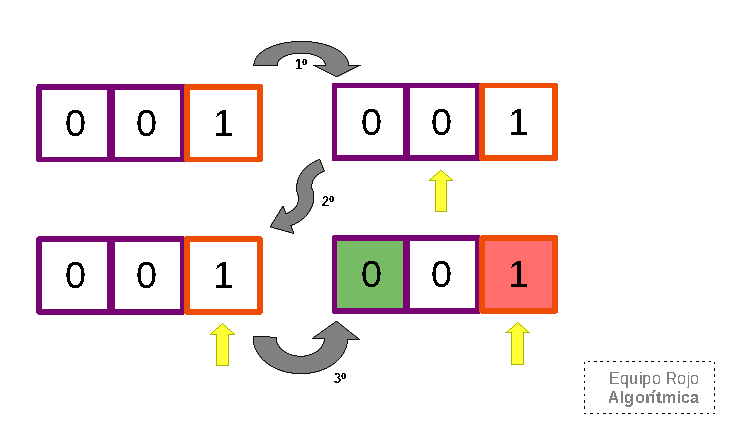
\includegraphics{img/esquema_fallo1a.pdf}
    \caption{Vector con elementos repetidos para el que falla 
    el algoritmo \ref{alg:1a-dyv}. Elaboración propia.}
    \label{fig:fallo-1a}
\end{figure}

Para solventar este problema, se ha de modificar el algoritmo \ref{alg:1a-dyv}, de manera que, cuando en una de las mitades
no encuentra un elemento que verifica la condición, también busque en la otra.

\subsubsubsection{Pseudocódigo}

\lstinputlisting[caption=Pseudocódigo asociado al caso Divide y Vencerás., label={alg:1b-dyv}]{listing/ejer1b-pseudo-dyv.txt}

\subsubsubsection{Implementación}

\lstinputlisting[language=C++, firstline=106, lastline=134, 
caption=Implementación en C++ del algoritmo basado en Divide y Vencerás., label={cod:1b-dyv}]
{../src/ejercicio-1-comp-fija-repetidos.cpp} 

\subsubsubsection{Determinación del umbral}

En este caso, a partir de los datos experimentales obtenidos en las tablas ?? y ??, y cuya representación
gráfica queda reflejado en ??, el tiempo de ejecución del algoritmo empleado Divide y Vencerás
es siempre mayor o igual que el tiempo empleado por el algoritmo obvio. Las \textbf{razones} de esta situación están
explicadas en \ref{sec:1b-comp}. Por tanto, tenemos que el \textbf{umbral} queda especificado en \ref{eq:1b-umbral}. 

\begin{equation}
    \boxed{UMBRAL \rightarrow +\infty}
    \label{eq:1b-umbral}
\end{equation}


Las repercusiones de este resultado quedan nuevamente discutidas en \ref{sec:1b-comp}.

\subsubsubsection{Análisis de Eficiencia}

El análisis de eficiencia \textbf{teórico} es análogo al realizado en \ref{sec:1a-dyv}, \textbf{con la salvedad} de que, en el
peor caso, se ha de explorar también la otra mitad del vector, por lo que la expresión \ref{eq:1a-efi-dyv-rec}
se transformaría en \ref{eq:1b-efi-dyv-rec} (con $c \in \mathbb N$ una constante). 

\begin{equation}
    T(n) = \left\{ \begin{array}{lr} 2 T(n/2) + c & \text{si } n > \text{UMBRAL}\\ n & \text{si } n \leqslant \text{UMBRAL} \end{array} \right.
    \label{eq:1b-efi-dyv-rec}
\end{equation}

Para resolver \ref{eq:1b-efi-dyv-rec}, para $n > \text{UMBRAL}$
consideramos el cambio
de variable $n = 2^k$, por lo que la expresión queda $T(2^k) = 2T(2^{k-1}) + c$. Haciendo
un nuevo cambio de variable $t_m = T(2^m)$, tenemos que:
$t_m = 2 t_{m-1} + c$. Tenemos que la ecuación característica
asociada a la homogénea es $x-2 = 0$ y una solución particular 
es $\{c_o\}$, con $c_o \in \mathbb R$ constante. Por tanto, $t_m = T(2^m) = c_0 + c_1 2^m$,
con $c_0, c_1 \in \mathbb R$, de donde deducimos que 

\begin{equation}
    T(n) = c_0 + c_1 n \Rightarrow \boxed{T(n) \in O(n)}
\end{equation}

Para la eficiencia \textbf{híbrida}...

\subsubsection{Comparativa} \label{sec:1b-comp}

Al contrario que en el caso de vectores no repetidos, comparando 
las tablas ?? y ?? y está representado en la gráfica ??, los \textbf{tiempos 
de ejecución son peores} en el caso Divide y
Vencerás que en el caso obvio. El origen de esto se debe a las siguientes
razones:

\begin{itemize}
    \item \textbf{Mismo orden de eficiencia}. Al contrario que en el caso con valores 
    no repetidos, el orden de eficiencia
    es la misma tanto en el caso obvio como en el caso trivial, tal y como se puede
    observar en la expresión \ref{eq:2a-eficiencia}, por lo que este resultado es plausible. 
    \item \textbf{Sobrecarga de la pila}. En los vectores generados, la distribución 
    general es la aparición del índice
    buscado en los elementos finales del vector, lo que obliga tanto al caso obvio como al caso
    Divide y Vencerás a analizar casi todo el vector, presentando éste último el 
    inconveniente de, en cada iteración, \textbf{introducir información de contexto
    en la pila} por cada llamada recursiva, lo que penaliza el rendimiento global del
    algoritmo. 
\end{itemize}

Como consecuencia de esta situación, tenemos que el algoritmo \ref{alg:1a-obvio} es siempre mejor o igual 
que el algoritmo \ref{alg:1b-dyv}, por lo que la técnica Divide y Vencerás \textbf{no logra superar en 
rendimiento} al caso obvio en ningún caso. Por tanto, en cualquier situación será más recomendable
implementar el caso obvio en lugar de emplear esta técnica. 